\section{Kalman Filters}

The concept of the Kalman filter was first published by Rudolph E. Kalman in 1960 in his paper “A new approach to linear filter and prediction problems”. Kalman sought to create a new method of estimating linear dynamic systems that was more practical to use with machine computation. Kalman explains, “Present methods for solving the Wiener problem (linear dynamic systems) are subject to a number of limitations which seriously curtail their practical usefulness.” [1] Kalman details his newly invented algorithm which provides efficient computational means to recursively estimate the state and error covariance of a process, in a way that minimizes the mean of the squared error covariance [2].

The algorithm, now dubbed the Kalman filter, is a set of mathematical equations broken up into two steps: Predict and Update.

\begin{figure}
    \centering
    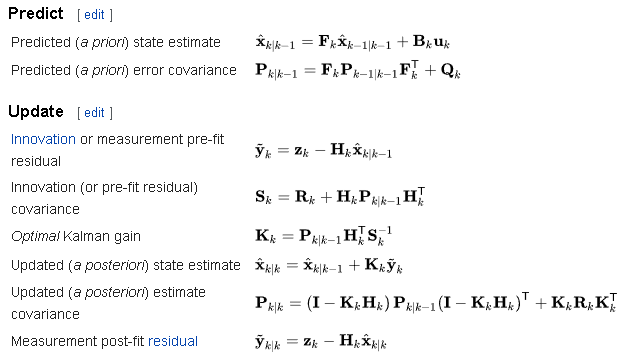
\includegraphics[width=12cm]{body/background/KFEqu.png}
    \caption{KF Equations}
    \label{fig:my_label}
\end{figure}

The predict step is used to predict the future values of the system with uncertainties. The update step updates the state and error covariance by computing a weighted average of the predicted value and the measured value know as the Kalman Gain. The Kalman Gain is then used to help determine the next predicted state of the Kalman filter. The algorithm continuously cycles through each step as more measure values at discrete time intervals (k to indicate a discrete time step and z$_k$ to indicate a measured value at time k) are recorded.
Today the Kalman filter is used in several modern applications such as sensor fusion/filtering, data smoothing, and forecasting/prediction [1] [3] [4] [5]. However, since this project is focused on forecasting tournament outcomes, the Kalman filter prediction applications will be explored. Kalman filters are well suited to predicting random signals such as tournament entries.  Kalman filters are capable of a dynamic model-based prediction [6]. The algorithm will recursively adapt the parameters of a selected model to best fit the trend of the entries. Contests with several discrete measurement points can by dynamically modelled in this fashion to result in a powerful prediction. Examples of Kalman filter forecasting can be found in several prediction algorithms such as slip model prediction for outdoor mobile robots, Seat geek’s ticket prices, and coal consumption [5] [7] [8]. The Kalman filter has also been improved to support non-linear models. The extended Kalman filter was developed by NASA Ames to solve nonlinear systems in flight navigation [9]. This was done substituting in differentiable functions for the predicted state estimate and innovation residual steps (discussed in the implementation section). Most of the contests are non-linear making the Kalman filter even more powerful for this application.
